\documentclass[12pt,a4paper]{article}

\usepackage[utf8]{inputenc}
\usepackage[ngerman]{babel}
\usepackage[T1]{fontenc}
\usepackage{amsmath}
\usepackage{amsfonts}
\usepackage{amssymb}
\usepackage{graphicx}
\usepackage[left=2cm,right=2cm,top=2cm,bottom=2cm]{geometry}
\usepackage{multicol}
\usepackage{booktabs}
\usepackage[hidelinks]{hyperref}
\usepackage{tikz}
\usepackage{pgfplots}
\usepackage{blindtext}
\usepackage{array}
\usepackage{multirow}
\usepackage{bigdelim}
\usepackage{colortbl}
\usepackage{fancyhdr} 
\usepackage{tabularx}
\usepackage{pgfplots}
\usepackage{xcolor}
\usepackage{amssymb}
\usepackage{color}
\usetikzlibrary{decorations.text}
\usetikzlibrary{tikzmark}
\pagestyle{fancy} 
	\fancyhf{} 
	\fancyhead[L]{
\includegraphics[scale=0.05]{Bilder/dhbw.png}} 
	\fancyhead[C]{\slshape Datenbanken} 
	\fancyhead[R]{\slshape LaTeX Version}
	\fancyfoot[C]{\thepage}

\usepackage{helvet}
\renewcommand{\familydefault}{\sfdefault}

\def\ojoin{\setbox0=\hbox{$\bowtie$}%
  \rule[-.02ex]{.25em}{.4pt}\llap{\rule[\ht0]{.25em}{.4pt}}}
\def\leftouterjoin{\mathbin{\ojoin\mkern-5.8mu\bowtie}}
\def\rightouterjoin{\mathbin{\bowtie\mkern-5.8mu\ojoin}}

\newcolumntype{Z}{>{\centering\let\newline\\\arraybackslash\hspace{0pt}}X}
\author{\slshape Robin Rausch, Florian Maslowski, Ozan Akzebe}
\title{Datenbanken}
\date{\slshape \today}
\begin{document}
\maketitle
\tableofcontents
\newpage
\section{Grundlagen}
	\subsection{Ebenen}
		\begin{description}
			\item[Interne:] wirkliche Speicherung der Daten im internen Speicher (SQL)
			\item[Konzeptionelle:] beschreibt welche Daten gespeichert werden sollen und wie die Beziehung der Daten untereinander aufgebaut ist. (ERM, UML)
			\item[Externe:] Sicht des Kunden auf die Daten. Hier kann für jede Benutzergruppe eine eigene Sicht auf die Daten zur Verfügung gestellt werden.
		\end{description}

	\subsection{Begrifflichkeiten}
	\begin{description}
		\item[Entität:] Entitäten einer Datenbank sind Objekte, die sich eindeutig von anderen Objekten des gleichen Entitätstyps abgrenzen lassen. Die Entitäten stehen in der Regel mit sich selbst oder mit anderen Entitäten in Beziehung.
		\item[Relation:] Tabelle, in welcher jedes Tupel  eine Entität darstellt.
		\item[Attribut:] In einem relationalen Datenbankmodell ist ein Attribut eine Spalte einer Tabelle. Jede Entität besitzt eine definierte Anzahl an Attributen (Eigenschaften), die sich eindeutig von anderen Entitäten des gleichen Entitättyps abgrenzen.
		\item[Beziehung:] Verbindung zwischen Entitäten. Gibt Kardinalitäten an
		\item[Tupel:] Zeile in Tabelle
		\item[Indizes:] Datenbankindex, welcher von der Datenstruktur getrennt ist. Beschleunigt Suche und Sortierung nach bestimmten Feldern
		\item[Optimizer:] Macht DB effizient. Sucht besten Weg eine Anfrage auszuführen. Indizes spielen eine wichtige Rolle.
		\item[Schema:] Struktur einer Tabelle. Gesammtheit der Attribute und deren Eigenschaften.
		\item[Instanz/Ausprägung:] Spezielle Ausprägung eines Schemas mit zugehörigen Werten
	\end{description}
	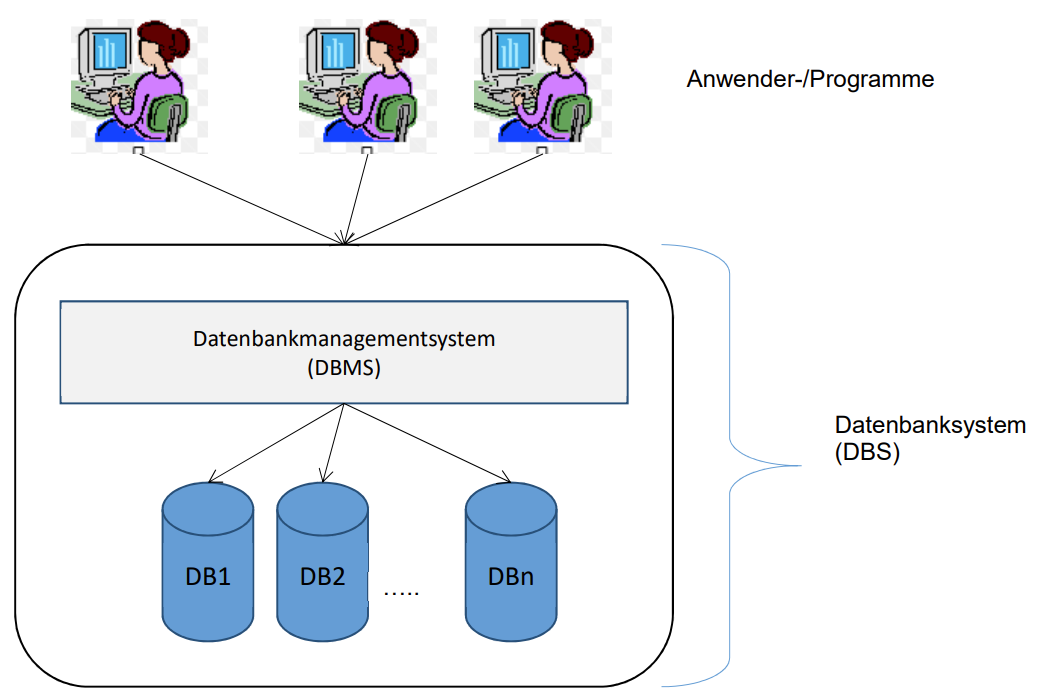
\includegraphics[width=0.6\textwidth]{Bilder/Begriffe.PNG}

	\subsection{Historie}
		\subsubsection{Hierarchisches Modell}
			Das Hierarchische Modell kann nur 1:N Beziehungen modellieren, da dieses wie eine Baumstruktur aufgebaut ist. 
		
		\subsubsection{Relationale Datenbanken}
			Bei Relationalen Datenbanken liegt der Fokus auf den Relationen. Hier können auch N:M Beziehungen modelliert werden.
			
	\subsection{Coddschen Regeln}
		\begin{description}
			\item[Integration:] Keine Dopplungen der Daten
			\item[Operation:] CRUD - create, read, update und delete 
			\item[Katalog:] Im Katalog werden Informationen abgelegt, die die Daten in einer Datenbank beschreiben.
			\item[Benutzersichten:] Daten können verschieden gelesen/interpretiert werden
			\item[Konsistenzüberwachung/Integritätssicherung:] Die Korrektheit der Daten muss zu jedem Zeitpunkt gewährleistet sein. Es dürfen keine Anomalien auftreten. Die Datenspeicherung muss nach einem vorgegebenen Schema erfolgen. 
			\item[Zugriffskontrolle:] Nur notwendige Personen sollen auf die Daten zugreifen können.
			\item[Transaktionen:] Bündelung mehrerer Anweisungen zu einer einzigen Transaktion, welche als eine funktionale Einheit ausgeführt werden – entweder ganz oder gar nicht.
			\item[Synchronisation:] Parallel ausgeführte Transaktionen müssen den gleichen Datenbankzustand hervorrufen wie irgendeine serielle Ausführung der Transaktionen.
			\item[Datensicherung:] Das Datenbanksystem muss nach einem Systemfehler in der Lage sein, den letzten konsistenten Datenbankzustand mittels automatischer Datensicherungs- und Wiederherstellungsmechanismen herzustellen.   
		\end{description}
			
	\subsection{Von der Idee zur Datenbank}
		\textbf{Vorgehen:}
		\begin{enumerate}
			\item Anforderungsanalyse
			\item Kozeptioneller Entwurf (ERM)
			\item Logischer Entwurf (Überführung des ERM in ein Datenbankmodell)
			\item Datenbank-Definition (DDL)\\ \textit{Kann zusammen mit Logischem Entwurf zu sog. \textbf{Implementierungsentwurf} zusammengefasst werden}
			\item Physikalischer Entwurf
		\end{enumerate}
		Ebenso muss das Sichtenmodell beachtet werden. Dieses beschreibt die Problematik, dass unterschiedliche Personen/Rollen unterschiedliche Sichten auf ein Modell haben. Bei der Planung müssen deshalb diese Sichten kombiniert werden, um eine universelle Lösung zu finden.

	\subsection{Referentielle Integrität}
		RI meint Bedingungen, die zur Sicherung der Datenintegrität bei Nutzung relationaler Datenbanken beitragen können. Nach der RI-Regel dürfen Datensätze (über ihre Fremdschlüssel) nur auf existierende Datensätze verweisen.

\section{Normalisierung}
	Dient dazu redundante Speicherung von Informationen und damit Inkonsistenz und Anomalien zu vermeiden.
	\subsection{Begrifflichkeiten}
		\begin{description}
			\item[Funktionale Abhängigkeit:] Attribut B ist voll funktional abhängig von A, wenn B durch A eindeutig identifiziert werden kann. ($f(A)=B$)
			\item[Triviale funktionale Abhängikeiten:] sind funktionale Abhängigkeiten auf sich selbst: $f(A)=B$ mit $B \subseteq A$ bzw. $X \rightarrow X$ 
			\item[Verlustfreie Zerlegung:] Alle Tupel der ursprünglichen Tabelle können durch einen Join aus den abgeleiteten Relationen wiederherstellen lassen. 
			Sie sichert damit die Wiederherstellbarkeit der ursprünglichen Relation.
			\item[Abhängigkeitsbewahrend:] Wenn alle Funktionalen Abhängigkeiten, nach Zerlegung der (Ursprungs)-Relation, auf einer der Teilrelationen dargestellt werden können.
		\end{description}

	\subsection{Schlüssel}
		\subsubsection{Superschlüssel}
			Jede Teilmenge $S_i \subseteq$ [R] für die gilt $S_i \rightarrow$ [R] heißt Superschlüssel von R.\\
			Ein Superschlüssel ist die Menge von Attributen einer Relation, welche ein Tupel in dieser Relation eindeutig identifizieren. Es sagt noch nichts darüber aus, ob es sich um eine minimale Menge von Attributen handelt. Ein Superschlüssel wäre zum Beispiel die Menge aller Attribute einer Relation gemeinsam ([R] $\rightarrow$ [R]).
		
		\subsubsection{Schlüsselkandidat}
			Eine minimale Teilmenge der Attribute eines Superschlüssels, welche die Identifizierung der Tupel ermöglicht (Schlüsselkandidaten $\subseteq $ Superschlüssel). In der Regel wird einer dieser Kandidaten als Primärschlüssel ausgewählt. Eine Relation kann mehrere Schlüsselkandidaten haben. 

		\subsubsection{Primärschlüssel}
			Der Primärschlüssel ist dann ein (willkürlich) ausgewählter Schlüsselkandidat, der zur eindeutigen Identifikation der Tupel in der Relation verwendet wird. 

		\subsubsection{Primattribute}
			Ein Attribut wird Primattribut oder prim genannt, wenn es in irgendeinem Schlüsselkandidaten von [R] vorkommt.\\
			Formal: Wenn K die Menge aller Schlüsselkandidaten von [R] ist, dann heißen alle Attribute in der Vereinigung über alle j von $K_j$, prim oder Primattribute.
			Alle Attribute in $\bigcup_j K_j$ heißen prim.

	\subsection{Normalformen}
	\subsubsection{1. Normalform}
		Eine Relation erfüllt die erste Normalform, wenn jede Entität (jedes Tupel) für jedes Attribut der Relation nur einen Datenwert besitzt.\\
		Atomar => Attribute können nicht weiter aufgeteilt werden.

	\subsubsection{2. Normalform}
		Eine Relation erfüllt die zweite Normalform (2NF), wenn diese sich in der ersten Normalform befindet und alle Nichtschlüsselattribute nur durch den gesamten Primärschlüssel festgelegt werden.\\
		Also: 1. Normalform + Nichtschlüsselattribute sind von jedem Schlüsselkandidaten voll funktional abhängig.\\
		Nichtschlüsselattribute müssen vom gesammten Schlüssel abhängig sein. Dazu müssen eventuell die Tabellen gesplittet werden.

	\subsubsection{3. Normalform}
		Eine Relation ist in der 3.Normalform (3NF), wenn diese die 2. Normalform erfüllte und keine transitiven Abhängigkeiten zwischen einem Nichtschlüsselattribut und einem Schlüsselkandidaten bestehen.\\
		Also: 2. Normalform + keine transitiven Abhängigkeiten von Nichtschlüsselattribut zu Schlüsselkandidat.\\
		Das heißt: Wenn B von A abhängig ist (A -> B), darf B nicht auf z.B. C abbilden(B->C). Hier müssen, die von B abhängigen Attribute in eine extra Tabelle ausgelagert werden. Dazu müssen eventuell die Tabellen gesplittet werden.\\
		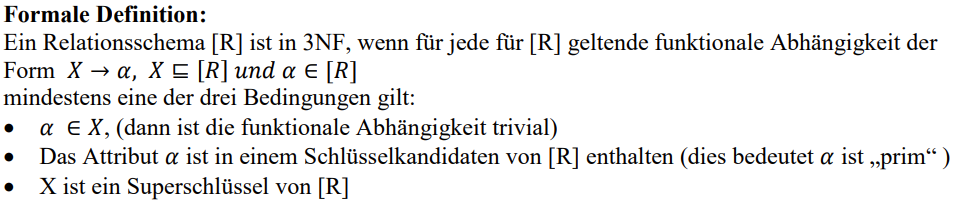
\includegraphics[width=\textwidth]{Bilder/3_nf.PNG}

	\subsubsection{Boyce-Codd Normalform}
		Die Boyce-Codd Normalform ist eine Verschärfung der 3NF. Die Boyce-Codd-Normalform (BCNF) ist eine Weiterentwicklung der Dritten Normalform (3NF). In der Dritten Normalform kann es vorkommen, dass ein Teil eines Schlüsselkandidaten funktional abhängig ist von einem Teil eines anderen Schlüsselkandidaten. Die Boyce-Codd-Normalform verhindert diese funktionale Abhängigkeit. \\
		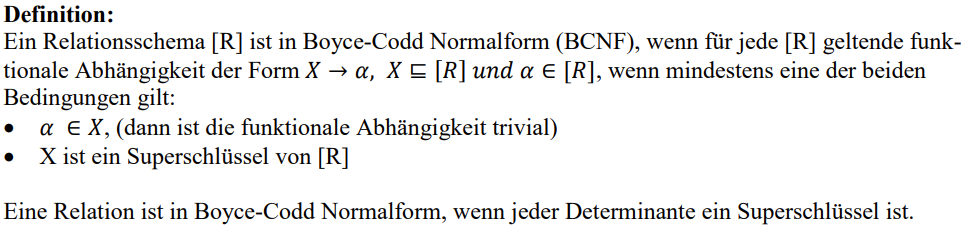
\includegraphics[width=\textwidth]{Bilder/boyce_codd.PNG}

	\subsection{Zerlegung/Dekomposition von Relationen}
		\includegraphics*[scale=1]{Bilder/RelSchema.png}\\\\
		Schlüsselkandidat ist nur $ad$.\\
		Zerlegung in mehrere Tabellen:\\
		R1: \underline{a, d}, f\\
		R2: \underline{d}, e\\
		R3: \underline{a}, b, c

		Da $[R1] \wedge [R2 = d]$ 

\section{Datenbankmanagementsystem (DBMS)}
	\subsection{PostgreSQL}
		\textcolor{red}{flo?}

	\subsection{MySql}
		\textcolor{red}{flo?}

\section{Entity Relationship Model}
	\subsection{Chen-Notation}
	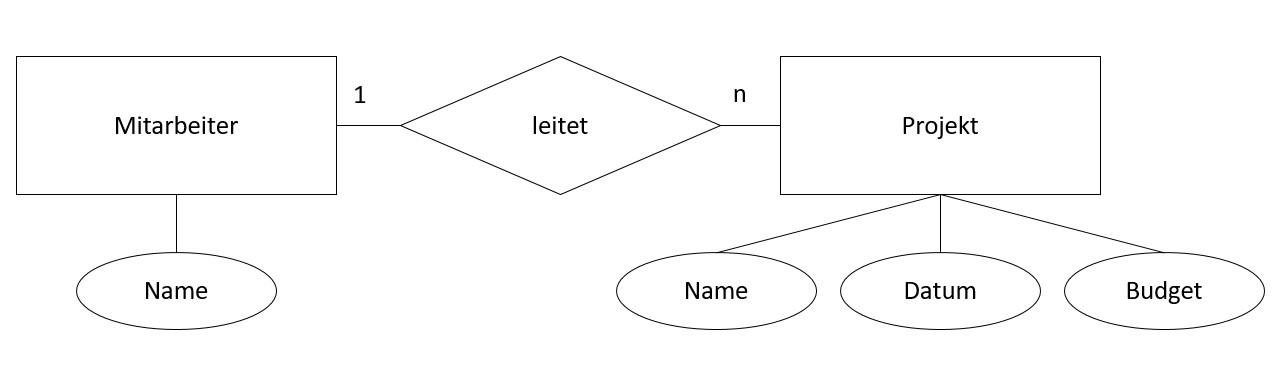
\includegraphics[width=\textwidth]{Bilder/chen.jpg}

	\subsection{Min-Max-Notation}
	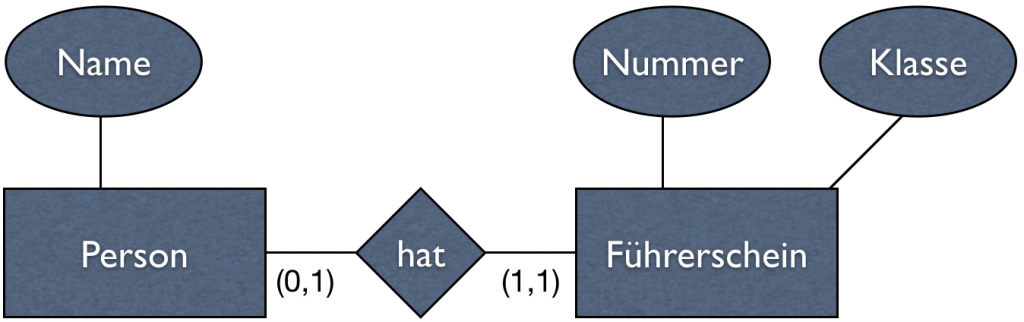
\includegraphics[width=\textwidth]{Bilder/min_max.png}

	\subsection{Krähenfß-Notation}
	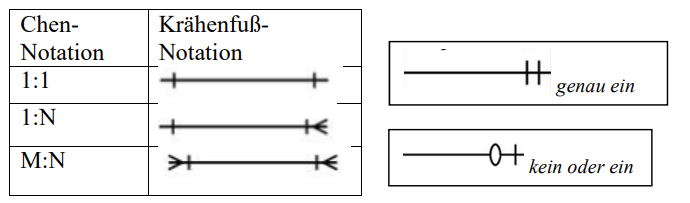
\includegraphics[width=0.6\textwidth]{Bilder/kraehenfuss1.PNG}
	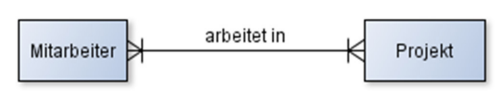
\includegraphics[width=0.4\textwidth]{Bilder/kraehenfuss2.PNG}

\section{SQL}
	SQL lässt sich in folgende Formen von Kommandos einteilen: \\
	Data Manipulation Language (DML), Data Definition Language (DDL), Data Control Language(DCL), Data Query Language (DQL), Transaction Control Language (TCL).\\
	SQL setzt sich aus folgenden Sprachen zusammen:
	\begin{itemize}
		\item Data Definition Language (DDL)
		\item Data Manipulation Language (DML)
		\item Data Control Language (DCL)
		\item Data Query Language (DQL)
		\item Transaction Control Language (TCL)
	\end{itemize}

	\subsection{Data Manipulation Language (DML)}
		\textbf{Merkspruch:} Sag Für Wen Geht Hilde Ohne Lippenstift.\\
		\textbf{Befehle:} SELECT, FROM, WHERE, GROUP BY, HAVING, ORDER BY, LIMIT
		\begin{description}
			\item[SELECT] [columns] (Funktionen wie: AVG, SUM, ... möglich)
			\item[FROM] [table]
			\item[WHERE] condition(s) (Wird auf individuelle Zeilen angewandt)
			\item[GROUP BY] [column]
			\item[HAVING] [condition] (Wird auf Gruppen angewandt, Funktionen können verwendet werden.)
			\item[ORDER BY] [column] ASC/DESC
			\item[LIMIT] [number of rows];
		\end{description}
		\par\noindent\rule{\textwidth}{0.4pt}
		\begin{description}
			\item[UPDATE] [columns]
			\item[SET] [$column_n = value_n$] 
			\item[WHERE] [condition];
		\end{description}
		\par\noindent\rule{\textwidth}{0.4pt}
		\begin{description}
			\item[INSERT INTO] [table] [(column$_1$, column$_2$, ...)]
			\item[VALUES] [$column_n = value_n$];
		\end{description}
		\par\noindent\rule{\textwidth}{0.4pt}
		\begin{description}
			\item[DELETE FROM] [table]
			\item[WHERE] [condition]; 
		\end{description}
		Zusätzlich gibt es Löschregeln. Diese sind CASCADE, RESTRICT und SET NULL. CASCADE löscht alle Einträge in jeder Tabelle die mit dem gelöschten Element in Verbindung stehen. RESTRICT verbietet das Löschen und SET NULL löscht das genannte Element und setzt alle Referenzen des gelöschten Elementes auf NULL.\\\\
		DISTINCT schließt doppelte Werte aus (SELECT DISTINCT Vorname FROM Mitarbeiter). Man kann auch Funktionen anwenden, welche z.B. den Durchschnitt berechnen (AVG, SUM, COUNT, MIN, MAX).
		
		\subsubsection{Unterabfragen}
			Select Vorname, Nachname, Gehalt from Mitarbeiter Where Gehalt > (Select Avg(Gehalt) from Mitarbeiter) Order By Gehalt;\\
			Diese müssen in Klammern stehen. Bei den Unterabfragen können auch Tabellen herauskommen. In diesem Fall muss ein Ausdruck davor gesetllt werden(ANY, ALL, EXISTS, IN).

	\subsection{Data Definition Language (DDL)}
		\begin{description}
			\item[CREATE TABLE] [table] 
			\item[][column$_n$] [datatype] [constraints];
		\end{description}
		\par\noindent\rule{\textwidth}{0.4pt}
		\begin{description}
			\item[ALTER TABLE] [table] 
			\item[][column$_n$] [datatype] [constraints];
		\end{description}
		\par\noindent\rule{\textwidth}{0.4pt}
		\begin{description}
			\item[DROP TABLE] [table];
		\end{description}


	\subsection{Begriffe, etc.}
		\begin{description}
			\item[CONSTRAINTS:] Beschränkungen/Bedingungen für Spalten (Bsp.: UNIQUE, NOT NULL, CHECK, FOREIGN KEY, PRIMARY KEY, etc.)
			\item[]  
		\end{description}

	\subsection{ACID-Regeln}
		\begin{description}
			\item[Atomicity:] Transaktionen müssen ganz oder garnicht ausgeführt werden
			\item[Consistency:] Datenbank muss nach Transaktionen einen gültigen Zustand annehmen. 
			Bei Fehlern wird vorheriger Zustand beibehalten.
			\item[Isolation:] Abfragen von verschiedenen Usern/Prozessen müssen voneinander abgegrenzt sein.
			\item[Durability:] Werte müssen nach Transaktionen dauerhaft gespeichert sein.   
		\end{description}

	\subsection{Relationale Algebra}
		\subsubsection{Selektion $\sigma$}
			$\sigma_{Abteilung=ANr}(Mitarbeiter \times Abteilung)$ oder $\sigma_{Geschlecht='w'}(Mitarbeiter)$\\
			Damit bekommt man alle Zeilen für welche das zutrifft. Vergleichbar mit WHERE.
			
		\subsubsection{Projektion $\pi$}
			$\pi_{Name, Abteilung}(Mitarbeiter)$\\
			Damit bekommt man nur die selektierten Attribute der jeweiligen Zeilen. Vergleichbar mit SELECT.

		\subsubsection{Verkettung}
			Diese Grundfunktionen lassen sich auch verketten:\\
			$\pi_{Vorname}(\sigma_{Geschlecht='w'}(Mitarbeiter))$

		\subsubsection{Vereinigung und Differenz}
			Vereinigung:\\
			$\pi_{Nachname}(Mitarbeiter) \cup \pi_{Nachname}(Kunde)$\\
			Differenz:\\
			$\pi_{Nachname}(Mitarbeiter) - \pi_{Nachname}(Kunde)$

		\subsubsection{Durchschnitt}
			Der Durchschnitt wird gleich verwendet wie die Vereinigung und Differenz. Dieser gibt alle Zeilen der Einträge zurück die nicht in beiden Tabellen liegen. Das Zeichen ist $\cap$.

		\subsubsection{Kreuzprodukt}
			$\sigma_{Mitarbeiter.Gehaltsstufe = Vergütungsgruppe.Gehaltsstufe}(Mitarbeiter \times Vergütungsgruppe)$
			
		\subsubsection{JOIN}
			Wird durch $\Join$ dargestellt.

		\subsubsection{Theta-Join $\Join_p$}
			Das Theta-Join ist eine Erweiterung des Kreuzprodukts, das zusätzliche Bedingungen verwendet, um die Verknüpfung von Zeilen in zwei Tabellen zu steuern. Es wird mit dem Operator $ \Join_p $ dargestellt.\\
			Syntax:\\
			$ \sigma_{Bedingung}(Tabelle_1 \Join_p Tabelle_2) $\\
			Beschreibung:\\
			Das Theta-Join kombiniert Zeilen aus zwei Tabellen, indem es die angegebene Bedingung überprüft. Nur die Zeilen, die die Bedingung erfüllen, werden im Ergebnis zurückgegeben.\\
			Beispiel:\\
			$ \sigma_{Tabelle_1.Spaltename = Tabelle_2.Spaltename}(Tabelle_1 \Join_p Tabelle_2) $\\
			Dieser Syntax führt das Theta-Join durch, indem es die Spalten Spaltename in $Tabelle_1$ und $Tabelle_2$ vergleicht und nur die Zeilen zurückgibt, in denen die Werte übereinstimmen.

		\subsubsection{Equi-Join $\Join_{[L],[R]}$}
			Der Equi-Join ist eine spezielle Form des Theta-Joins, bei dem die Bedingung auf einer Gleichheit zwischen zwei Spalten basiert. Es wird häufig verwendet, um Zeilen aus zwei Tabellen basierend auf übereinstimmenden Werten in den angegebenen Spalten zu verknüpfen.\\
			Syntax:\\
			$\sigma_{Tabelle_1.Spaltename = Tabelle_2.Spaltename}(Tabelle_1 \Join_{[L],[R]} Tabelle_2)$\\
			Beschreibung:\\
			Der Equi-Join vergleicht die Werte der angegebenen Spalten in $Tabelle_1$ und $Tabelle_2$ und gibt nur die Zeilen zurück, in denen die Werte übereinstimmen.\\
			Beispiel:\\
			$\sigma_{Tabelle_1.ID = Tabelle_2.ID}(Tabelle_1 \Join_{[ID],[ID]} Tabelle_2)$

		\subsubsection{Natürlicher Join}
			Der Natürliche Join ist eine spezielle Form des Equi-Joins, bei dem die Verknüpfung basierend auf allen gemeinsamen Spaltennamen in den beiden Tabellen erfolgt. Es werden automatisch die Spalten verglichen, die den gleichen Namen haben.\\
			Syntax:\\
			$Tabelle_1 \Join Tabelle_2$\\
			Beschreibung:\\
			Der Natürliche Join vergleicht automatisch alle gemeinsamen Spalten in $Tabelle_1$ und $Tabelle_2$ und gibt nur die Zeilen zurück, in denen die Werte in allen gemeinsamen Spalten übereinstimmen.\\
			Beispiel:\\
			$Tabelle_1 \Join Tabelle_2$

		\subsubsection{Left Outer-Join}
			Der Left Outer-Join ist eine Verknüpfungsoperation, die alle Zeilen der linken Tabelle und die übereinstimmenden Zeilen der rechten Tabelle zurückgibt. Wenn keine Übereinstimmungen vorhanden sind, enthält das Ergebnis NULL-Werte für die Spalten der rechten Tabelle.\\
			Syntax:\\
			$Tabelle_1 \leftouterjoin Tabelle_2$ ON Bedingung\\
			Beispiel:\\
			$Mitarbeiter \leftouterjoin Abteilung$ ON Mitarbeiter.Abteilung = Abteilung.ANr\\
			Dieser Syntax führt einen Left Outer-Join durch, indem er die Spalte Abteilung in der Tabelle Mitarbeiter mit der Spalte ANr in der Tabelle Abteilung vergleicht und alle Zeilen der Tabelle Mitarbeiter und übereinstimmende Zeilen der Tabelle Abteilung zurückgibt.
			
		\subsubsection{Right Outer-Join}
			Der Right Outer-Join ist eine Verknüpfungsoperation, die alle Zeilen der rechten Tabelle und die übereinstimmenden Zeilen der linken Tabelle zurückgibt. Wenn keine Übereinstimmungen vorhanden sind, enthält das Ergebnis NULL-Werte für die Spalten der linken Tabelle.\\
			Syntax:\\
			$Tabelle_1 \rightouterjoin Tabelle_2$ ON Bedingung\\
			Beispiel:\\
			$Mitarbeiter \rightouterjoin Abteilung$ ON Mitarbeiter.Abteilung = Abteilung.ANr\\
			Dieser Syntax führt einen Right Outer-Join durch, indem er die Spalte Abteilung in der Tabelle Mitarbeiter mit der Spalte ANr in der Tabelle Abteilung vergleicht und alle Zeilen der Tabelle Abteilung und übereinstimmende Zeilen der Tabelle Mitarbeiter zurückgibt.\\

		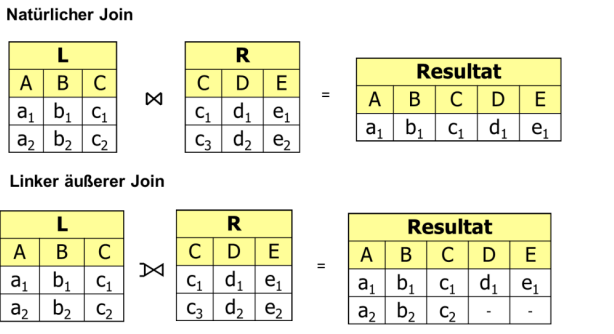
\includegraphics[width=0.5\textwidth]{Bilder/join1.PNG}
		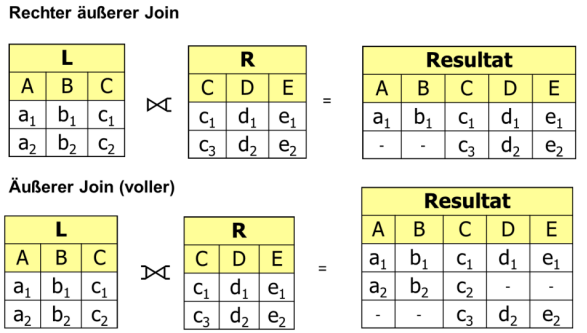
\includegraphics[width=0.5\textwidth]{Bilder/join2.PNG}

		\subsubsection{Umbenennung}
			Wird durch $\rho$ dargestellt. Die Umbenennung einer Relation kann dann erforderlich werden, wenn wir in einer Abfrage eine Relation mehrfach verwenden möchten (siehe Joins).
			
	\subsection{Views}
		Views in Datenbanken sind virtuelle Tabellen, die aus den Daten einer oder mehrerer Basis- oder anderen Views erstellt werden. Sie bieten eine Möglichkeit, Daten aus verschiedenen Tabellen logisch zu kombinieren oder bestimmte Daten aus einer Tabelle auszuwählen und sie als separate Tabelle darzustellen. Views stellen eine abstrahierte Sicht auf die zugrunde liegenden Daten dar, wobei die tatsächlichen Daten unverändert bleiben.\\
		Views bieten mehrere Vorteile. Erstens ermöglichen sie eine verbesserte Datenintegrität, da sie es ermöglichen, komplexe Regeln und Einschränkungen auf die darunterliegenden Tabellen anzuwenden. Zweitens ermöglichen Views eine verbesserte Sicherheit, da sie den Zugriff auf sensible Daten einschränken können, indem sie nur bestimmte Spalten oder Zeilen zugänglich machen. Drittens erleichtern sie die Datenbankverwaltung, da sie komplexe Abfragen vordefinieren und die Wiederverwendung von Abfragen ermöglichen.\\
		Views können in Abfragen genauso verwendet werden wie reguläre Tabellen. Benutzer können auf sie zugreifen, Daten abfragen, Aktualisierungen durchführen oder sie in anderen Views verwenden. Änderungen, die an den Daten einer View vorgenommen werden, können sich auf die zugrunde liegenden Tabellen auswirken, je nach den festgelegten Regeln und Einschränkungen.\\
		Zusammenfassend bieten Views in Datenbanken eine flexible und effiziente Möglichkeit, Daten logisch zu organisieren, komplexe Abfragen zu vereinfachen, die Sicherheit zu verbessern und die Datenintegrität zu gewährleisten.

	\subsection{Transaktionen}
		Eine Transaktion ist eine logische Arbeitseinheit (Bündelung mehrerer Anweisungen), welche dafür sorgt, dass logisch zusammengehörige Folgen von Operationen ohne negative Begleiterscheinungen auf der Datenbank ausgeführt werden können. Transaktionen folgen ebenfalls den ACID Anforderungen. Verhindern dass zwei gleichzeitig auftretende Anfragen an eine Datenbank die Integrität zerstören oder falsche Ergebnisse liefern. Sobald ein Fehler bei einer Transaktion auftritt, wird ein Rollback ausgeführt der die Änderungen rückgängig macht.

\end{document}